\section{Охорона праці і навколишнього середовища}
\subsection{Аналіз умов праці на робочому місці}
Розділ виконано для етапу розробки на ЕОМ MacBook Pro (15-inch, 2018).

Робота проводилась на кафедрі <<Програмної інженерії та Інформаційних Технологій Управління>>, яка розташована на сьомому поверсі семи поверхової будівлі.

Обладнання, приміщення і режим праці користувача повинні відповідати вимогам наступних нормативно-технічних документів:
\begin{enumerate}
	\item НПАОП 0.00-7.15-18. Вимоги щодо безпеки та захисту здоров’я працівників під час роботи з екранними пристроями.
	\item ДСанПіН 3.3.2.007-98. Державні санітарні правила і норми роботи з візуальними дисплейними терміналами електронно-обчислювальних машин.
	\item ДСТУ Б В.1.1-36:2016. Визначення категорій приміщень, будинків та зовнішніх установок за вибухопожежною та пожежною небезпекою.
	\item ДБН В.1.1-7-2016. Пожежна безпека об’єктів будівництва. Загальні вимоги.
	\item ДСН 3.3.6.042-99. Санітарні норми мікроклімату виробничих приміщень.
	\item ДБН В.2.5-67:2013. Опалення, вентиляція та кондиціонування.
	\item ДБН В.2.5-28-2018. Природне та штучне освітлення.
	\item ДСН 3.3.6.037-99. Санітарні норми виробничого шуму, ультразвуку та інфразвуку.
	\item ГОСТ 12.1.029-80 ССБТ. Средства и методы защиты от шума. Классификация.
	\item ДСТУ ГОСТ 12.1.012:2008. Вібраційна безпека. Загальні вимоги.
	\item ДСН 3.3.6.039-99. Санітарні норми виробничої загальної та локальної вібрації.
	\item ДСТУ ГОСТ 2656885:2009. Вібрація. Методи і засоби захисту. Класифікація.
	\item ДСТУ ГОСТ 12.1.038:2008. Електробезпека. Гранично допустимі рівні напруг дотику і струмів.
	\item ПУЕ. Правила улаштування електроустановок.
	\item НПАОП 40.1-1.32-01. Правила будови електроустановок. Електрообладнання спеціальних установок.
	\item ДСТУ ГОСТ 7237:2011. Електробезпека. Загальні вимоги та номенклатура видів захисту.
	\item ГОСТ 14254-96. Степени защиты, обеспечиваемые оболочками.
	\item НАПБ А.01.001-2014. Правила пожежної безпеки в Україні.
	\item ДСТУ БВ.2.5-38:2008. Інженерне обладнання будинків і споруд. Улаштування блискавка захисту будівель і споруд (IEC 62305:2006, NEQ).
	\item НАПБ Б.06.004-2005. Перелік однотипних за призначенням об’єктів, які підлягають обладнанню автоматичними установками пожежа гасіння та пожежної сигналізації.
	\item ГН 3.3.5-8.6.6.1-2014. Гігієнічна класифікація праці за показниками шкідливості та небезпечності факторів виробничого середовища, важкості та напруженості трудового процесу.
\end{enumerate}

Загальна характеристика виробничого приміщення, в якому виконувалась робота, приведена у таблиці~\ref{tab:labor_1}.

В таблиці~\ref{tab:labor_2} надано перелік потенційних небезпечних та шкідливих факторів на робочому місці користувача ЕОМ з монітором на рідинних кристалах.

\subsection{Захист від шкідливого впливу факторів виробничого середовища}
Захист від шкідливого впливу факторів виробничого середовища
Підтримка оптимальних параметрів мікроклімату в робочій зоні здійснюється відповідно вимог ДБН В.2.5-67:2013 за допомогою кондиціонеру, який регулює температуру повітря. Передбачена можливість природнього провітрювання приміщення. У холодний період року проводиться опалення від центральної тепломережі.%~\cite{Labor29}.

{
\footnotesize
\tabulinesep=1.2mm
\begin{longtabu} to \textwidth {|X[1,l]|X[3,l]|X[3,l]|X[3,l]|X[3,l]|X[3,l]|}
	\caption{Характеристика виробничого приміщення }
	\label{tab:labor_1} \\
	\hline
	№ п/п & Найменування показника & Характеристика показника & Обґрунтування вибору значення показника & Документ, що регламентує цій показник & Примітка \\
	\hline
	\endfirsthead
	\caption*{Закінчення таблиці \thetable{}}\\
	\hline
	№ п/п & Найменування показника & Характеристика показника & Обґрунтування вибору значення показника & Документ, що регламентує цій показник & Примітка \\
	\hline
	\endhead

	1 & 2 & 3 & 4 & 5 & 6 \\ \hline

	\multirow{2}{*}{1} & Розміри приміщення (м); & 4х5,3х3,3 & \multirow{2}{=}{На одне р.м. з ЕОМ не менше 6.0 $\textup{м}^2$ площі} & \multirow{2}{=}{ДСанПіН 3.3.2-007-98} & \multirow{2}{=}{Фактично 2.5-3 $\textup{м}^2$ на одне р.м. з ЕОМ, що відповідає нормі} \\ \cline{2-3}
	& Кількість робочих місць (р.м.) & 8 & & & \\ \hline

	\multirow{3}{*}{2} & \multirow{2}{=}{Природне освітлення, вікна виходять на південний схід} & \multirow{2}{=}{Бокове, одностороннє; азимут 135˚} &  Див. таблицю~\ref{tab:labor_2} & ДБН В.2.5-28-18 & \\ \cline{4-6}
	& & & КПО не нижче 1.5\% & ДСанПіН 3.3.2-007-98 & Для р.м. з ЕОМ \\
	& & & & &  \\ \hline

	\multirow{2}{*}{3} & \multirow{2}{=}{Штучне освітлення, кількість світильників N;  джерела світла} & \multirow{2}{=}{Загальне рівномірне; N=5; люмінесцентні лампи} & Див. таблицю~\ref{tab:labor_2} & ДБН В.2.5-28-18	& \\ \cline{4-6}
	& & & Не нижче 300-500 лк & ДСанПіН 3.3.2-007-98 & Для робочих місць з ЕОМ \\
	& & & & &  \\
	& & & & &  \\ \hline

	4 & Характеристика трифазної електричної мережі & Чотири провідна з глухо заземленою нейтраллю напругою 380/220 В, частотою 50 Гц & Довгі кабельні мережі великої ємності & ПУЕ & \\ \hline

	5 & Клас приміщення за ступенем небезпеки ураження електрострумом & З підвищеною небезпекою & Є можливість одночасного дотику до металоконструкцій будівлі, що мають з'єднання з землею, та до металевих корпусів ЕОМ & ПУЕ & Необхідно передбачити заходи безпеки згідно вимог ПУЕ \\ \hline

	6 & Категорія приміщення з вибухо-пожежної небезпеки & В & Є тверді спаленні матеріали: папір, деревина тощо & ДСТУ Б В.1.1-36:2016 & \\ \hline

	7 & Ступінь вогнестійкості будівельних конструкцій & ІІ & 7-и поверхова будівля; категорія В & ДБН В.1.1.7−2016	& \\ \hline

\end{longtabu}
}

{
\footnotesize
\tabulinesep=1.2mm
\begin{longtabu} to \textwidth {|X[1,l]|X[3,l]|X[3,l]|X[3,l]|X[3,l]|X[3,l]|}
	\caption{Перелік потенційних шкідливих та небезпечних факторів на робочому місці користувача ЕОМ з ЖК монітором}
	\label{tab:labor_2} \\
	\hline
	№ & Назва фактора & Джерела виникнення & Умови роботи & Нормативні параметри, їх значення & Документ, що регламентує показник \\
	\hline
	\endfirsthead
	\caption*{Закінчення таблиці \thetable{}}\\
	\hline
	№ & Назва фактора & Джерела виникнення & Умови роботи & Нормативні параметри, їх значення & Документ, що регламентує показник \\
	\hline
	\endhead

	1 & 2 & 3 & 4 & 5 & 6 \\ \hline

	\multicolumn{6}{|l|}{І. Небезпечні фактори} \\ \hline

	1 & Висока електрична напруга & Мережа живлення устаткування & Нормальний режим роботи & Струм $I_h = 0.3$ мА; Напруга $U_{\textup{дот}} < 2 \textup{В}$ & ДСТУ ГОСТ 12.1.038:08 \\ \hline

	\multicolumn{6}{|l|}{ІІ. Шкідливі фізичні фактори} \\ \hline

	2 & Несприятливе освітлення & Стан систем природного та штучного освітлення & МРОР 0,3-0,5 мм; розряд ІІІ; підрозряд <<в>>, фон середній, контраст середній & КПО $D_{\min}^{\textup{н сум}} = 1.2\%$; освітленість $E_{\min} = 300 \textup{лк}$ & ДБН В.2.5-28-18 \\ \hline

	3 & Несприятливий мікроклімат: температура ($t$), відносна вологість ($\phi$), швидкість руху ($v$) & Стан систем опалення та вентиляції & Категорія важкості робіт Іа; холодний період & Оптимальні:
	$t$ -- 22-24˚C;
	$\phi$ -- 40-60\%;
	$v$ -- не більше 0.1 м/с & ДСН 3.3.6.042-99 \\ \hline

	4 & Підвищений рівень шуму & Кондиціонери кулери, системи освітлювання, перетворювачі напруги, принтери & Творча діяльність, програмування & Рівень звуку $L_A = 50\textup{ дБА}$ & ДСН 3.3.6.037-99 \\ \hline

	5 & Вібрація & & Загальна технологічна, категорія 3, тип <<в>>, умови комфорту & Рівень віброшвидкості $L_V = 75\textup{ дБ}$ & ДСТУ ГОСТ 12.1.012:08, ДСН 3.3.6.039-99 \\ \hline

	6 & Психо-фізіологічна перенапруга & Монотонність праці, розумова напруга, статичність і незручність пози & & 1 та 2 клас умов праці для напруженості і важкості трудового процесу & ГН 3.3.5-8.6.6.1-2014 \\ \hline

\end{longtabu}
}

Згідно ДСН 3.3.6.042-99, у приміщеннях із значними площами засклених поверхонь передбачаються заходи щодо захисту:
\begin{itemize}
	\item від перегрівання при попаданні прямих сонячних променів в теплий період року (орієнтація віконних прорізів схід -- захід, улаштування лоджій, жалюзі, сонцезахисних плівок та інше);
	\item від радіаційного охолодження --- в зимовий (використання стін певної товщини, подвійних стекол).
\end{itemize}

Робочі місця повинні бути віддалені від стін на відстань не менше 1 м.

Визначений в таблиці~\ref{tab:labor_2} коефіцієнт природного освітлення реалізується через вікна визначеної площини, яка розраховується при проектуванні будівлі, а нормований показник штучного освітлення ($E_{\min}$) реалізується шляхом встановлення визначеної кількості світильників і вибором потужності ламп в них.

Згідно вимог ДСанПіН 3.3.2.007-98, в разі штучного освітлення як джерела світла мають застосовуватись переважно люмінісцентні лампи типу ЛБ і світильники серії ЛПО3б із дзеркальними гратами, укомплектовані високочастотними пускорегулювальними апаратами (ВЧ ПРА).

Система загального освітлення має становити суцільні або преривчасті лінії світильників, розташовані збоку від робочих місць (переважно ліворуч), паралельно лінії зору працюючих. Слід передбачити обмеження прямої блискості від джерел природного та штучного освітлення та обмежувати відбиту блискість на робочих поверхнях. Необхідно чистити вікна і світильники не менше двох разів на рік та вчасно заміняти перегорілі лампи.%~\cite{Labor30}.

Заходи захисту від шуму та вібрації повинні відповідати вимогам ГОСТ 12.1.029-80 і ДСТУ ГОСТ 2656885:2009. Устаткування, що є джерелом шуму, слід розташовувати поза приміщенням для роботи з ЕОМ. Для забезпечення допустимих рівнів шуму у виробничих приміщеннях слід застосовувати засоби звукопоглинання, наприклад, перфоровані плити, панелі, підвісні стелі.

Як захист від шуму, який створюється вентиляторами системних блоків, використовується звукоізоляційний корпус. Вентилятор можна замінити на більш якісний або на мідні радіатори з водяним охолодженням. Крім того встановлюють перехідник з регулятором напруги і швидкості обертання процесорного кулеру, а при монтажі кулерів металеві гвинти заміняють гумовими пробками, що дозволяють ізолювати вентилятор від корпусу. Якщо принтер розташований на твердій поверхні, то для зменшення вібрації потрібно підстелити під нього щільний прогумований килимок.

\subsection{Електробезпека}
Персональна ЕОМ є однофазним споживачем електроенергії, який живиться від трифазної чотирьох провідної мережі перемінного струму напругою 380/220 В частотою 50 Гц з глухо заземленою нейтраллю.

У разі випадкового дотику до струмопровідних частин, що знаходяться під напругою, або появі напруги дотику на металевих кожухах електроустаткування, наприклад, при пошкодженні ізоляції можливі нещасні випадки в результаті дії електричного струму.

Клас пожежа небезпечної зони приміщення, згідно ПУЕ та НПАОП 40.1-1.32-01, −П-ІІа, бо у приміщенні знаходяться тверді спаленні матеріали.

Для приміщень з підвищеною небезпекою поразки людини електричним струмом ПУЕ передбачені конструктивні, схемно-конструктивні й експлуатаційні міри електробезпеки (ДСТУ ГОСТ 7237:2011):%~\cite{Labor31}:
\begin{itemize}
	\item Експлуатаційні міри. Необхідно дотримуватися правил безпеки при роботі з високою напругою і використовувати наступні запобіжні заходи, що передбачені НПАОП 0.00-7.15-18: не підключати і не відключати кабелю, якщо обладнання знаходиться під напругою; технічне обслуговування і ремонтні роботи виконувати тільки при вимкнутому живленні в мережі; встановлювати у приміщенні загальний вимикач для відключення електроустаткування. Забороняється залишати працюючу апаратуру без нагляду.
	\item Конструктивні заходи. ЕОМ відноситься до електроустановок до 1000 В закритого виконання, усі струмоведучі частини знаходяться в кожухах. Вибираємо ступінь захисту оболонки від зіткнення персоналу із струмоведучими частинами усередині захисного корпуса і від потрапляння води усередину корпусу ІP-44, де перша <<4>> --- захист від твердих тіл, розміром більш 1.0 мм, друга <<4>> --- захист від бризків води (ГОСТ 14254-96).
	\item Як схемно-конструктивна міра безпеки застосовується подвійна ізоляція (для монітору), малі напруги до 42 В, занулення (так як мережа живлення до 1000 В з глухо заземленою нейтраллю). Відповідно ДСТУ ГОСТ 7237:2011, занулення --- це навмисне електричне з'єднання металевих неструмоведучих частин комп'ютера, які у випадку аварії можуть виявитися під напругою, з нульовим захисним провідником.
\end{itemize}

Вихідні дані для розрахунку занулення однофазних споживачів (варіант 24):
\begin{equation*}
	P_1 = 525\textup{ Вт}, P_2 = 16000\textup{ Вт},
\end{equation*}
\begin{description}
	\item[де] $P_1$ --- потужність однофазного споживача електроенергії, наприклад, електронно-обчислювальної машини (ЕОМ), Вт;
	\item $P_2$ --- потужність усіх споживачів, які живляться від цього фазового провідника (кондиціонери, вентилятори, освітлювальні прилади, інші ЕОМ, принтери, тощо), кВт.
\end{description}
\begin{equation*}
	l_1 = 55\textup{ м}, l_2 = 138\textup{ м},
\end{equation*}
\begin{description}
	\item[де] $l_1$ --- довжина ділянки 1, м;
	\item $l_2$ --- довжина ділянки 2, м.
\end{description}
\begin{equation*}
	U_{\textup{л}} = 380\textup{ В}, U_{\textup{ф}} = 220\textup{ В},
\end{equation*}
\begin{description}
	\item[де] $U_{\textup{л}}$ --- лінійна напруга;
	\item $U_{\textup{ф}}$ --- фазова напруга.
\end{description}

Матеріал провідників -- алюміній, спосіб прокладки проводів на ділянці 1 -- металеві труби, на ділянці 2 -- земля. 

Занулення використовується в чотири провідних трифазових мережах із заземленою нейтраллю напругою до 1000 В. 
Схема мережі до розрахунку занулення зображена на рис.~\ref{fig:labor_nullation}.

\begin{figure}[H]
	\centering
	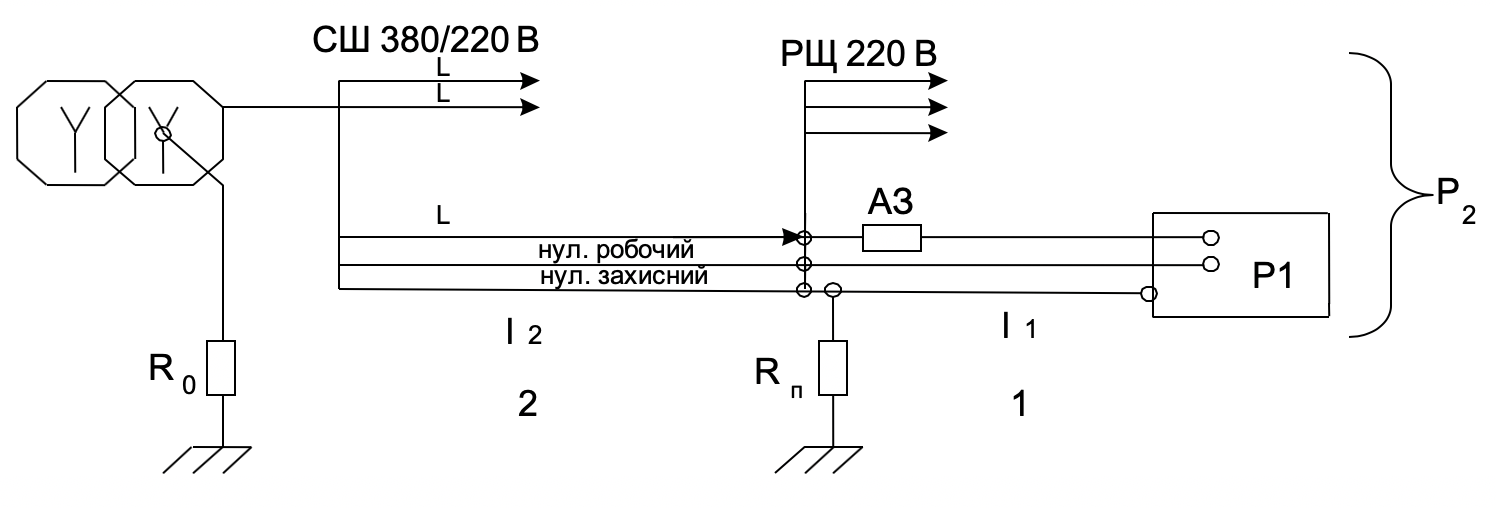
\includegraphics[width=0.8\textwidth]{labor_nullation}
	\caption{Схема мережі до розрахунку занулення}
	\label{fig:labor_nullation}
\end{figure}
\begin{description}
	\item[де] $T_{\textup{р}}$ --- масляний трансформатор, що понижує напругу з $U_1 = 6-10$ кВ до $U_2 = 380$ В, схема з'єднання обмоток --- зірка-зірка;
	\item ЗШ --- збірна шина;
	\item РЩ --- розподільний щит;
	\item АЗ --- апарат захисту;
	\item 1 --- лінія, що живить електроустановку потужністю $Р_1$;
	\item 2 --- живильний магістральний кабель.
\end{description}

Мета розрахунку --- визначення такого перерізу нульового захисного провідника, при якому струм короткого замикання (ІК) у задане число разів (К) перевищить номінальний струм апарату захисту ($I^{\textup{АЗ}}_{\textup{НОМ}}$), що забезпечить селективне відключення споживача, тобто повинна виконуватися умова:
\begin{equation} \label{eq:lab_check}
	I_{\textup{К}} \geq K \cdot I^{\textup{АЗ}}_{\textup{НОМ}}.
\end{equation}
\begin{description}
	\item[де] $K$ --- запас надійності.
\end{description}

Електромережа, що живіть комп'ютер та інші однофазні електроустановки, виконується як групова три провідна лінія шляхом прокладання фазового, нульового робочого і нульового захисного провідників з міді або алюмінію. Якщо кількість ЕОМ не перевищує 5 і вони розташовані по периметру приміщення, кабель в оболонці з неспалених матеріалів прокладають по підлозі вздовж стін. Якщо кількість ЕОМ перевищує 5 або вони розташовані у центрі приміщення, кабель прокладають у металевих трубах та гнучких металевих рукавах з відводами.

Нехай струм $I_1$, що живить електроустановку (ЕУ) потужністю $Р_1$, Вт:
\begin{equation*}
	I_1 = \cfrac{P_1}{U_{\textup{ф}}} = \cfrac{525}{220} = 2.3863, \textup{A}.
\end{equation*}

Струм $I_2$, що живить електроустановку (ЕУ) потужністю $Р_2$, Вт:
\begin{equation*}
	I_2 = \cfrac{P_2}{U_{\textup{ф}}} = \cfrac{16000}{220} = 72.7272, \textup{A}.
\end{equation*}

Визначення пускового струму $I_{\textup{пуск}}$ потужністю $P_1$, Вт:
\begin{equation*}
	I_{\textup{пуск}} =\cfrac{K_n}{K_T} I_1, \textup{A}.
\end{equation*}
\begin{description}
	\item[де] $K_n$ --- коефіцієнт кратності пускового струму, 2\dots7.5;
	\item $K_T$ --- коефіцієнт важкості пуску, залежить від часу пуску, 1.6\dots2.5; $K_T = 1.6$, якщо час пуску понад 10 с --- тяжкий пуск; $K_T = 1.6$, якщо час пуску дорівнює 10 с --- середній пуск; $K_T = 2.5$ якщо час пуску дорівнює 5 с --- легкий пуск.
\end{description}

Для ЕОМ $K_n = 3, K_T = 2.5$, тоді:
\begin{equation*}
	I_{\textup{пуск}} =\cfrac{3}{2.5} 2.3863 = 2.8635, \textup{A}.
\end{equation*}

Номінальний струм, при якому спрацьовує апарат захисту, повинен перевищувати $І_\textup{пуск}$, інакше апарат захисту буде спрацьовувати при кожному вмиканні електроустановки.

Для ЕОМ можна вибрати запобіжник типу ВПШ. Згідно із розрахунків $I_{\textup{пуск}}$, можна використовувати ВПШ значення якого вище $2.8635$ А, а саме ВПШ 6-11 з $I^{\textup{АЗ}}_{\textup{НОМ}} = 3.15$ А.

Струм короткого замикання $I_\textup{к}$, визначаємо за формулою:
\begin{equation} \label{eq:lab_ik}
	I_\textup{к} = \cfrac{U_\textup{ф}}{
		\cfrac{Z_{TP}}{3} + Z_{\textup{ПФН}}
	}, \textup{А},
\end{equation}
\begin{description}
	\item[де] $Z_{TP}$ --- повний опір трансформатора, Ом;
	\item $Z_{\textup{ПФН}}$ --- повний опір петлі фаза-нуль, Ом.
\end{description}

Величина $Z_{TP}$ залежить від потужності трансформатора, конструктивного виконання, напруги і схеми з¢єднання його обмоток (зіркою або трикутником).

Потужність трансформатора визначається за формулою:
\begin{equation*}
	N_{TP} = 4 \cdot P_2 = 4 \cdot 16 = 64, \textup{кВт}.
\end{equation*}

Вибираємо трансформатор потужністю 100 кВт, $Z_{TP} = 0.799$ Ом.

Повний опір петлі фаза-нуль визначається за формулою:
\begin{equation*}
	Z_{\textup{ПФН}} = \sqrt{(R_\textup{Ф} + R_\textup{НЗ})^2 + X^2}, \textup{Ом},
\end{equation*}
\begin{description}
	\item[де] $R_\textup{Ф}$ --- активний опір фазового захисного провідника, Ом;
	\item $R_\textup{НЗ}$ --- активний опір нульового захисного провідника, Ом.
\end{description}

Індуктивний опір петлі фаза-нуль $X$ визначається за формулою:
\begin{equation*}
	X = X_\textup{Ф} + X_\textup{НЗ} + X_\textup{ВЗ}, \textup{Ом},
\end{equation*}
\begin{description}
	\item[де] $X_\textup{Ф}$, $X_\textup{НЗ}$ --- внутрішні індуктивні опори фазового і нульового провідників, відповідно, Ом;
	\item $X_\textup{ВЗ}$ --- зовнішній індуктивний опір, який зумовлено взаємоіндукцією петлі фаза-нуль, Ом.
\end{description}

Для мідних та алюмінієвих провідників $X_\textup{Ф}$ та $X_\textup{НЗ}$ порівняно малі (близько $0.0156$ Ом/км), тому ними можна знехтувати.

Зовнішній індуктивний опір $X_\textup{ВЗ}$ залежить від відстані між проводами $D$ та їхнього діаметру $d$. Якщо нульові захисні проводи прокладають спільно з фазовими, значення $D$ мале й порівняльне з діаметром $d$, тому опір $X_\textup{ВЗ}$ незначний (не більш $0.1$ Ом/км) і ним можна знехтувати. Тоді:
\begin{equation*}
	Z_{\textup{ПФН}} = R_\textup{Ф} + R_\textup{НЗ}.
\end{equation*}

Таким чином первинна формула розрахунку~\eqref{eq:lab_ik} приймає вид:
\begin{equation*}
	I_\textup{к} = \cfrac{U_\textup{ф}}{
		\cfrac{Z_{TP}}{3} + R_\textup{Ф} + R_\textup{НЗ}
	}, \textup{А},
\end{equation*}

Визначимо значення активного опору фазового провідника за формулою:
\begin{equation} \label{eq:lab_r}
	R_{\textup{Ф}} = R_\textup{Ф1} + R_\textup{Ф2},
\end{equation}
\begin{description}
	\item[де] $R_\textup{Ф1}$, $R_\textup{Ф2}$ --- опір фазового провідника на ділянках 1 та 2, відповідно, Ом.
\end{description}

Для провідників з кольорових металів:
\begin{equation*}
	R_{\textup{Ф1}} = \cfrac{\rho\cdot l_1}{S_\textup{Ф1}}, \textup{Ом},
\end{equation*}
\begin{equation*}
	R_{\textup{Ф2}} = \cfrac{\rho\cdot l_2}{S_\textup{Ф2}}, \textup{Ом},
\end{equation*}
\begin{description}
	\item[де] $\rho$ --- питомий опір, $\cfrac{\textup{Ом} \cdot \textup{мм}^2}{\textup{м}}$, який дорівнює для міді $0.018$, а для алюмінію $0.028$;
	\item $S_\textup{Ф1}$, $S_\textup{Ф2}$ --- перерізи фазового провідника для ділянок 1 та 2, відповідно, $\textup{мм}^2$.
\end{description}

Перерізи фазових проводів визначають при проектуванні електричної мережі струму в залежності від величини струму, який проходить по проводам, умов прокладання кабелю, матеріалу провідників і т.п. Так згідно із вихідними даними значення перерізів дорівнюють:
\begin{equation*}
	S_{\textup{Ф1}} \approx 2, S_{\textup{Ф2}} \approx 7.
\end{equation*}

Опір фазових провідників дорівнюють:
\begin{equation*}
	R_{\textup{Ф1}} = \cfrac{\rho\cdot l_1}{S_\textup{Ф1}} = \cfrac{0.028 \cdot 55}{2} = 0.77, \textup{Ом},
\end{equation*}
\begin{equation*}
	R_{\textup{Ф2}} = \cfrac{\rho\cdot l_2}{S_\textup{Ф2}} = \cfrac{0.028 \cdot 138}{7} = 0.552, \textup{Ом}.
\end{equation*}

Визначення опору нульового захисного провідника:
\begin{equation*}
	R_{\textup{НЗ}} = R_{\textup{НЗ1}} + R_{\textup{НЗ2}}, \textup{Ом},
\end{equation*}
\begin{description}
	\item[де] $R_{\textup{НЗ1}}$, $R_{\textup{НЗ2}}$ --- опір нульового захисного провідника на ділянках 1 та 2, відповідно, Ом.
\end{description}

Площа перерізу нульового робочого та нульового захисного провідників в груповій три провідній мережі повинна бути не менш площі фазового провідника, тобто: $S_\textup{НЗ1} = S_\textup{Ф1}$, $S_\textup{НЗ2} = S_\textup{Ф2}$.
Відповідно, $S_\textup{НЗ} = S_\textup{Ф}$.

Обчислимо опір фазового провідника~\eqref{eq:lab_r}:
\begin{equation*}
	R_{\textup{НЗ}} = R_{\textup{Ф}} = R_{\textup{Ф1}} + R_{\textup{Ф2}} = 1.322, \textup{Ом},
\end{equation*}
отже:
\begin{equation*}
	I_\textup{к} = \cfrac{220}{
		\cfrac{0.799}{3} + 1.322 + 1.322
	} = \cfrac{220}{2.9103} = 75.5927, \textup{А}.
\end{equation*}

Перевірка виконання умов надійності та ефективності роботи занулення.
Повинно виконуватися співвідношення~\eqref{eq:lab_check}, де $K = 3$ для запобіжників:
\begin{equation*}
	75.5927 \geq 3 \cdot 3.15.
\end{equation*}

Утрати напруги на ділянках 1 та 2 не повинні перебільшувати 22 В:
\begin{gather*}
	U_\textup{П1} + U_\textup{П2} \leq 22, \textup{В}, \\
	U_\textup{П1} = I_1 \cdot R_\textup{Ф1} = 2.3863 \cdot 0.77 = 1.8374, \textup{В}, \\
	U_\textup{П2} = I_2 \cdot R_\textup{Ф2} = 72.7272 \cdot 0.552 = 40.1454, \textup{В}, \\
	40.1454 + 1.8374 \leq 22.
\end{gather*}

Виходячи з розрахунків, друга умова не виконується і треба обрати більше значення для перерізу фазового провідника для ділянки 2, так як вона має велику утрату напруги.

Беручи $S_\textup{Ф2} = 14$ повторимо розрахунки:
\begin{gather*}
	R_{\textup{Ф2}} = \cfrac{\rho\cdot l_2}{S_\textup{Ф2}} = \cfrac{0.028 \cdot 138}{14} = 0.276, \textup{Ом}, \\
	U_\textup{П2} = I_2 \cdot R_\textup{Ф2} = 72.7272 \cdot 0.276 = 20.0727, \textup{В}, \\
	20.0727 + 1.8374 \leq 22.
\end{gather*}

Всі умови виконуються. Таким чином були обрані:
\begin{itemize}
	\item запобіжник ВПШ 6-11;
	\item перерізи фазового та нульового захисного провідників для першої ділянки 2 $\textup{мм}^2$;
	\item перерізи фазового та нульового захисного провідників для першої ділянки 14 $\textup{мм}^2$.
\end{itemize}

\subsection{Пожежна безпека}
У зв'язку з поширенням комп’ютерної техніки, що може привести до загоряння, треба передбачати можливі наслідки і розробляти заходи щодо їх попередження. Причинами загоряння стають: несправність електричного обладнання, пошкодження ізоляції, коротке замикання кола струму, перегрів проводів, поганий контакт в місцях з'єднання; розряди статичної електрики, які особливо небезпечні в вибухонебезпечних приміщеннях, блискавка.

Пожежна безпека забезпечується наступними мірами:
\begin{enumerate}[label={\arabic*)}]
	\item системою запобігання пожеж;
	\item системою пожежного захисту;
	\item організаційними заходами щодо пожежної безпеки.
\end{enumerate}

Система запобігання пожеж передбачає запобігання утворенню пального середовища і запобігання утворенню в пальному середовищі джерел запалювання.

Для зменшення небезпеки утворення в пальному середовищі джерел запалювання передбачено:
\begin{enumerate}[label={\arabic*)}]
	\item використання електроустаткування, що відповідає класу пожежа небезпечної зони приміщення П-ІІа за ПУЕ та НПАОП 40.1-1.32-01: ступінь захисту електроапаратури не менш ІP-44, ступінь захисту світильників ІР-2Х;
	\item використання електроустаткування, що відповідає класу пожежа небезпечної зони приміщення П-ІІа за ПУЕ та НПАОП 40.1-1.32-01: ступінь захисту електроапаратури не менш ІP-44, ступінь захисту світильників ІР-2Х;
	\item забезпечення захисту від короткого замикання (контроль і профілактика ізоляції, використання запобіжників);
	\item вибір перетину провідників по максимально допустимому нагріванню;
	\item будівлі, в яких встановлено обладнання інформаційних технологій чи будь-яке інше електронне обладнання, чутливе до атмосферних перешкод, незалежно від кількості уражень об'єктів за рік потребує І або ІІ рівня блискавка захисту (ДСТУ БВ.2.5-38:2008).
\end{enumerate}

Система протипожежного захисту призначена для локалізації та гасіння пожежі. При виборі засобів гасіння пожежі для забезпечення безпеки людини від можливості поразки електричним струмом у приміщенні відповідно вимог НАПБ А.01.001-2014 передбачено використання вуглекислотних вогнегасникiв ВВК-5. Вогнегасник знаходиться на видному і легко доступному місці. При виникненні пожежі передбачені можливості аварійного відключення апаратури і комунікацій та повідомлення в пожежну охорону по телефону. У якості сповіщувачів використовуються система автоматичної пожежної сигналізації відповідно вимог НАПБ Б.06.004-2005. Ступінь вогнестійкості будинку згідно ДБН В.1.1-7-2016 --- ІІ. У приміщенні є два незалежних виходи для евакуації людей під час пожежі.

Організаційними заходами протипожежної профілактики є вступний інструктаж при надходженні на роботу, навчання виробничого персоналу протипожежним правилам, видання необхідних інструкцій і плакатів, засобів наочної агітації, наявність плану евакуації.%~\cite{Labor32}.

\subsection{Охорона навколишнього середовища}
Закон України <<Про охорону навколишнього середовища>> від 25 червня 1991р. --- закон, що визначає правові, економічні та соціальні основи організації охорони природи навколишнього природного середовища в інтересах нинішнього і майбутніх поколінь.

Закон встановлює, що завданням законодавства про охорону навколишнього природного середовища є регулювання відносин у галузі охорони, використання і відтворення природних ресурсів, забезпечення екологічної безпеки, запобігання і ліквідації негативного впливу господарської та іншої діяльності на навколишнє природне середовище, збереження природних ресурсів, генетичного фонду живої природи, ландшафтів та інших природних комплексів, унікальних територій та природних об'єктів, пов'язаних з історико-культурною спадщиною.

Збільшення використання енергії призводить до порушення екологічної рівноваги природного середовища, яке складалася століттями. 

Поряд з цим, підвищення технічної оснащеності підприємств, застосування нових матеріалів, конструкцій і процесів, збільшення швидкостей і потужностей виробничих машин впливають на навколишнє середовище.

При масовому використанні моніторів та комп’ютерів не можна не враховувати їхній вплив на навколишнє середовище на всіх стадіях --- при виготовленні, експлуатації та після закінчення терміну служби.

Міжнародні екологічні стандарти, що діють на сьогоднішній день в усьому світі, визначають набір обмежень до технологій виробництва та матеріалів, які можуть використовуватися в конструкціях пристроїв. Так, за стандартом ТСО-95, вони не повинні містити фреонів (турбота про озоновий шар), полівінілхлориді, бромідів (як засобів захисту від загоряння).

У стандарті ТСО-99 закладене обмеження за кадмієм у світлочутливому шарі екрана дисплея та ртуті в батарейках; э чіткі вказівки відносно пластмас, лаків та покриттів, що використовуються. Поверхня кнопок не повинна містити хром, нікель та інші матеріали, які визивають алергічну реакцію. ГДК пилу дорівнює $0.15 \textup{мг/м}^3$, рекомендовано $0.075 \textup{мг/м}^3$; ГДК озону під час роботи лазерного принтеру --- $0.05 \textup{мг/м}^3$. Особливо жорсткі вимоги до повторно використовуваних матеріалів.

Міжнародні стандарти, починаючи з ТСО-92, включають вимоги зниженого енергоспоживання та обмеження припустимих рівнів потужності, що споживаються у неактивних режимах.
Дотримання приведених нормативних параметрів небезпечних і шкідливих виробничих факторів дозволить забезпечити більш здорові і безпечні умови роботи користувача ЕОМ.

